\documentclass[11pt]{article}
\usepackage{amsmath}
\usepackage{newpxtext}
\usepackage{lipsum}
\usepackage{float}
\usepackage{enumerate}
\usepackage{subfigure}
\usepackage{geometry}
\usepackage{graphicx}
\usepackage{booktabs}
\usepackage{makecell}
\usepackage{amssymb}
\usepackage[dvipsnames]{xcolor}
\usepackage{multirow}

\usepackage{tikz}
\usepackage{pgfplots}
\pgfplotsset{compat=1.18}

\setcounter{secnumdepth}{4}
\geometry{a4paper,scale=0.85}
\linespread{1}

% change subtitle format
\usepackage{titlesec}
\titleformat{\section}{\Large\bfseries}{\textcolor{Blue}{Week\,{\thesection}}}{1em}{\hspace{0em}}{}
\titleformat{\subsection}{\large\bfseries}{\textcolor{Blue}{\S\,{\thesubsection}}}{1em}{\hspace{0em}}{}
\titleformat{\subsubsection}{\bfseries}{\textcolor{Blue}{\S\,{\thesubsubsection}}}{1em}{\hspace{0em}}{}

\begin{document}

\begin{center}
    \begin{large}
        \textbf{Computational Neuroscience}
    \end{large}
\end{center}
\tableofcontents

\newpage
\section{Course Introduction and Basic Neurobiology}
\subsection{Descriptive, Mechanistic and Interpretive Models}
\begin{enumerate}
    \item Descriptive models (\textbf{What}): describe ways that a neuron respond to external stimuli; encoding (describe responses), decoding (extract information)
    \item Mechanistic models (\textbf{How}): simulating single/a network of neurons
    \item Interpretive (Normative) models (\textbf{Why}): explaining the behaviour of neurons and neural networks
\end{enumerate}
\noindent \textbf{Receptive fields}: Specific region or sensory space in which a stimulus can incur an electrical response in a sensory neuron.

(1) Descriptive
\begin{itemize}
    \item How visual information is received: visual information$\rightarrow$ retina (ganglion cells)$\rightarrow$ lateral geniculate nucleus (LGN)$\rightarrow$ primary visual cortex (v1)
    \begin{center}
        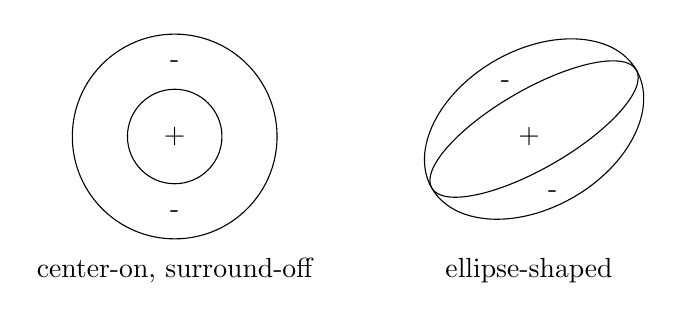
\begin{tikzpicture}
            \draw (0, 0) circle (1.3cm);
            \draw (0, 0) circle (0.6cm);
            \node[] at (0, 0) {+};
            \node[] at (0, 0.95) {-};
            \node[] at (0, -0.95) {-};
            \node[] at (0, -1.7) {center-on, surround-off};
            \draw[rotate=30] (4, -2.2) ellipse (1.5cm and 1cm);
            \draw[rotate=30] (4, -2.2) ellipse (1.5cm and 0.5cm);
            \node[] at (4.5, 0) {+};
            \node[] at (4.2, 0.7) {-};
            \node[] at (4.8, -0.7) {-};
            \node[] at (4.5, -1.7) {ellipse-shaped};
        \end{tikzpicture}
    \end{center}
    \item The receptive fields are modeled by \textbf{reverse correlation}.
\end{itemize}

(2) Mechanistic: How are receptive fields constructed? (from LGN to primary visual cortex)
\begin{itemize}
    \item Hubel \& Wiesel: v1 RFs are constructed from converging LGN inputs
    \begin{center}
        \centering
        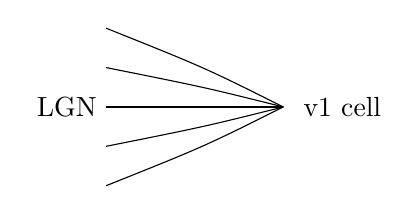
\begin{tikzpicture}
            \tikzstyle{every node}=[font=\normalsize]
            \node [font=\normalsize] at (2.5,11.75) {LGN};
            \node [font=\normalsize] at (6,11.75) {v1 cell};
            \draw (3,11.75) .. controls (4.25,11.75) and (4.25,11.75) .. (5.25,11.75);
            \draw (3,12.25) .. controls (4.25,12) and (4.25,12) .. (5.25,11.75);
            \draw (3,11.25) .. controls (4.25,11.5) and (4.25,11.5) .. (5.25,11.75);
            \draw (3,10.75) .. controls (4.25,11.25) and (4.25,11.25) .. (5.25,11.75);
            \draw (3,12.75) .. controls (4.25,12.25) and (4.25,12.25) .. (5.25,11.75);
        \end{tikzpicture}
    \end{center}
    \item \textcolor{Blue}{\textbf{Controversial}}: The hypothesis does not take into account other recurrent inputs
\end{itemize}

(3) Descriptive: Why do we need receptive fields?
\begin{itemize}
    \item \textcolor{Blue}{\textbf{Efficient Coding Hypothesis}}: the brain's goal is to represent images as faithfully and efficiently as possible using receptive fields. Let $RF_i$ denote the $i$th receptive field:
    \begin{align*}
        &\hat{I} = \sum_{i=1}^N RF_i\omega_i\\
        &\min \ \frac{1}{N}\sum_{i=1}^N (\hat{I}-I)^2
    \end{align*}
    Our brain adjusts the weights regarding each receptive field $\omega_i$ to minimize mean square error.
    \item Efficient coding algorithms: sparse coding, ICA, predictive coding; starting with random $RF_i$ and run until convergence.
\end{itemize}

\subsection{Neurobiology Fundamentals}
\noindent \textbf{The Neuron Doctrine}
\begin{itemize}
    \item Neuron is the fundamental structural and functional unit of the brain.
    \item Neurons are discrete cells and not continuous with other cells.
    \item Information flows from the dendrites to the axon via the cell body.
\end{itemize}
\subsubsection{Action Potential}
EPSP refers to excitatory postsynaptic potential. When $\sum \text{EPSP}\geq \text{threshold}$, action potential, or output spike, is generated.

\begin{enumerate}
    \item Identities of cell membrane
    \item Neuron Signaling 
    \begin{itemize}
        \item spikes from presynaptic neurons $\rightarrow$ chemically gated channels open (at synapses) $\rightarrow$ changes in local membrane potential
        \item $\rightarrow$ voltage-gated channels $\rightarrow$ reaches action potential\\
        depolarization (voltage increases), hyperpolarization (voltage decreases)
    \end{itemize}

        \begin{center}
        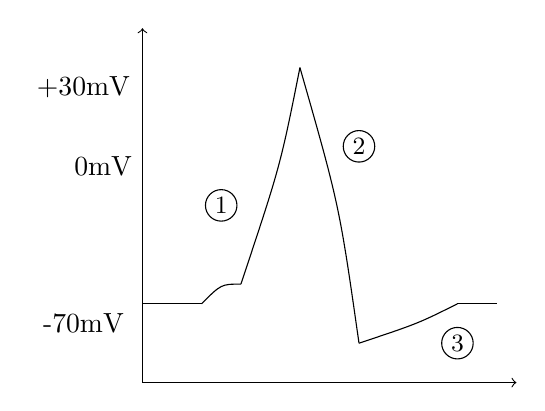
\begin{tikzpicture}
            \tikzstyle{every node}=[font=\normalsize]
            \draw[->]  (4,8.25) .. controls (4,10.5) and (4,10.5) .. (4,12.75);
            \draw[->]  (4,8.25) .. controls (6.5,8.25) and (6.5,8.25) .. (8.75,8.25);
            \draw  (4,9.25) .. controls (4.5,9.25) and (4.5,9.25) .. (4.75,9.25);
            \draw  (4.75,9.25) .. controls (5,9.5) and (5,9.5) .. (5.25,9.5);
            \draw (5.25,9.5) .. controls (5.75,11) and (5.75,11) .. (6,12.25);
            \draw  (6,12.25) .. controls (6.5,10.5) and (6.5,10.5) .. (6.75,8.75);
            \draw  (6.75,8.75) .. controls (7.5,9) and (7.5,9) .. (8,9.25);
            \draw  (8,9.25) .. controls (8.25,9.25) and (8.25,9.25) .. (8.5,9.25);
            \node [font=\normalsize] at (3.25,12) {+30mV};
            \node [font=\normalsize] at (3.5,11) {0mV};
            \node [font=\normalsize] at (3.25,9) {-70mV};
            \draw  (5,10.5) circle (0.2cm) node {\small 1} ;
            \draw  (6.75,11.25) circle (0.2cm) node {\small 2} ;
            \draw  (8,8.75) circle (0.2cm) node {\small 3} ;
        \end{tikzpicture}
    \end{center}
    \makebox{\textbf{Stage 1}} Chemically-gated channels activated; voltage-gated channels activated, sodium channels open with Na$^+$ ions rushing into the neuron.\par
    \makebox{\textbf{Stage 2}} Sodium channels inactivated and potassium channels open (K$^+$ ions rushing out)\par
    \makebox{\textbf{Stage 3}} Potassium channels close, sodium-potassium pumps open using ATP
    \item Mylination of axons: action potential hops from non-mylinated regions\\
    Active wiring: enable lossless signal propagation (saltatory conduction)
\end{enumerate}

\subsubsection{Synapses}
There are two types of junctions between neurons:
\begin{itemize}
    \item \textit{Electrical synapses}: Gap junctions enable direct connection between neurons which lead to fast and rapid \textcolor{Blue}{\textbf{synchronization}}.
    \item \textit{Chemical synapses}: Neurotransimitter molecules are received by receptors, or the chemically-gated channels. This junction enables optionally connected ionic channles and more \textcolor{Blue}{\textbf{modifiable communication}}.
\end{itemize}
The table below shows what occurs to postsynaptic membranes in exitatory or inhibitory synapses.
\begin{table}[H]
    \centering
    \begin{tabular}{|c|c|c|}
    \hline
    \begin{tabular}[c]{@{}c@{}}Membrane/\\ Synapse Type\end{tabular} & \begin{tabular}[c]{@{}c@{}}Presynaptic\\ Membrane\end{tabular} & \begin{tabular}[c]{@{}c@{}}Postsynaptic\\ Membrane\end{tabular} \\ \hline
    Excitatory Synapse   {{(1)}}                                               & \multirow{2}{*}{$\rightarrow$}                                 & potential +                                                     \\ \cline{1-1} \cline{3-3} 
    Inhibitory Synapse                                               &                                                                & potential $-$                                                     \\ \hline
    \end{tabular}
\end{table}
In (1), excitatory postsynaptic potential is generated (what we known as EPSP).
\\

\noindent \textbf{The Synapses Doctrine}: basis for memory and learning
\begin{itemize}
    \item \textcolor{Blue}{\textbf{Hebbian plasticity}}: If neuron $A$ repeatedly fires neuron $B$, the synapse from $A$ to $B$ is strengthened, which indicates a faster response.
    \item \textit{Long Term Potentiation} (LTP) and \textit{Long term Depression} (LTD) refers to the experimentally observed change in EPSP size or the same input over time. LTP and LTD strongly depends on spike sequence and timing: ``Those who fire together, wire together''
    
    \begin{center}
        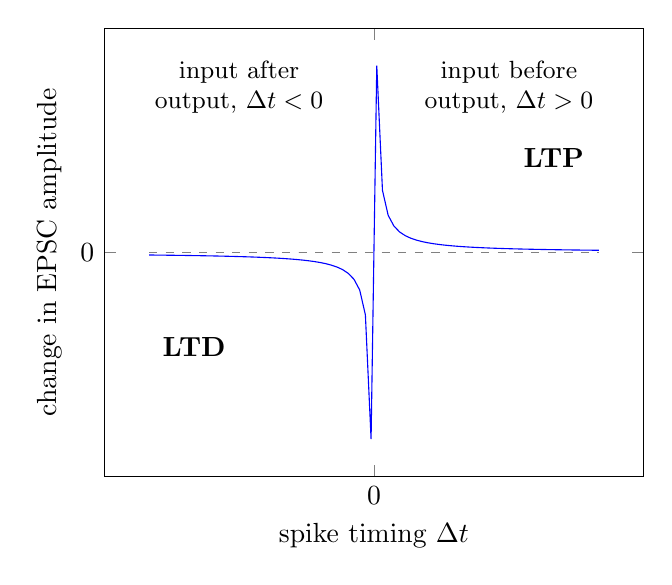
\begin{tikzpicture}
            \begin{axis}[xlabel={spike timing $\Delta t$},
                ylabel={change in EPSC amplitude},
                xtick={0},
                ytick={0}]
                \addplot[color=blue, 
                domain=-10:10, 
                samples=80]{1/x};
                \addplot[color=gray, dashed, domain=-10:10]{0};
                \node[] at (axis cs:-8,-4) {\textbf{LTD}};
                \node[] at (axis cs:8,4) {\textbf{LTP}};
                \node[] at (axis cs:6,7) {\small \makecell{input before \\ output, $\Delta t>0$}};
                \node[] at (axis cs:-6,7) {\small \makecell{input after \\ output, $\Delta t<0$}};
            \end{axis}
        \end{tikzpicture}
    \end{center}
\end{itemize}

\subsubsection{Brain Areas, Networking and Functions}
The nervous system incorporates \textit{peripheral system} and \textit{central nervous system}.
\begin{itemize}
    \item Peripheral nervous system (PNS)
    \begin{enumerate}
        \item \textbf{Somatic}: nerves connecting to voluntary skeletal muscles and sensory receptors. \\
        Afferent nerve fibres transmit signals from periphery to CNS; Efferent nerve fibres work the opposite way.
        \item \textbf{Autonomic}: nerves that connect to the heart, blood vessels, smooth muscles and glands.
    \end{enumerate}
    \item Central nervous system (CNS) = spinal cord + brain
\end{itemize}
\textbf{Comparisons between biological brain and digital computer}
Due to the parallel computation and adaptive connectivity of biological brains, they are better at ill-posed problems such as speech and vision. For digital computers, they excel in math and symbol processing with sequential information processing with fixed connectivity of CPUs.

\newpage
\section{Neural Encoding Models}
\subsection{The Neural Code}
\begin{itemize}
    \item \textbf{Neural Coding} performs the characterization of the hypothetical relationship between stimulus and neuronal responses, and the relationship among the electrical activities of neurons in the ensemble.  The subject of investigation can be described as $\mathbb{P} (\text{response}\,|\,\text{stimumus})$, or, how does a stimulus cause a pattern of responses? 
    \item \textbf{Raster Plot} is a tool for recording neuronal responses (spikes) with a given stimulus. The figure below shows a sample raster plot with the behavior of different neurons.
    \begin{center}
        \begin{tikzpicture}
            % Draw axes
            \draw[->] (0,0) -- (8,0) node[right] {Time};
            \draw[->] (0,0) -- (0,4) node[above] {Neuron};
        
            % Define spikes for each neuron (manually set)
            % Neuron 1 spikes
            \foreach \x in {1, 2.5, 4.7, 7.5, 8.2}
                \draw (\x,1) -- (\x,1.5);
            % Neuron 2 spikes
            \foreach \x in {0.5, 1.5, 3.5, 6.5, 9}
                \draw (\x,2) -- (\x,2.5);
            % Neuron 3 spikes
            \foreach \x in {2, 3, 5, 7, 8}
                \draw (\x,3) -- (\x,3.5);
            % Add more neurons as needed
            
            % Label neurons
            \foreach \y/\ytext in {1.25/1, 2.25/2, 3.25/3}
                \node at (-0.5,\y) {\ytext};
        \end{tikzpicture}
    \end{center}
    \item When we observe action potentials, or, spikes in a particular situation, the neurons are responding to external stimulus by \textbf{encoding features}. 
    \item \textbf{Tuning curves}: The y-axis of these curves are usually average firing rate, and the x-axis represents the stimulus parameter. It can be the orientation angle of the stimulus, the intensity of lighting on our subject of investigation, movement directions or anything.
    \item The neural codes demonstrate increasing levels of complexity when the stimulus parameter becomes more closely aligned with realistic scenarios. For example, fundamental geometric shapes can be perceived by simple receptive fields, while portrait and sceneries might involve more complicated stimulus representations. From morphological features to semantic implications, firing behavior becomes increasingly abstract along with the rise in complexity of the receptive fields.
    \item Neural Code Conclusion
    \begin{enumerate}
        \item Neural coding translates the neuronal responses into specific forms for further investigation.
        \item Creating raster plots is an easy way to record and represent action potentials. 
        \item Neural codes become increasingly absract when the complexity of receptive field rises. For instance, semantic expressions usually have a more intricate nature.
    \end{enumerate}
\end{itemize}

\subsection{Basic Encoding Models}
\begin{enumerate}
    \item \textbf{Subject of investigation}: $\mathbb{P}$(response|stimulus)
    \item Simplest linear mapping
    \begin{align*}
        r(t)=\phi s(t)
    \end{align*}
    \item Temporal filters
    \begin{align*}
        &r(t)=\sum_{k=0}^n s_{t-k}f_k\\
        &r(t)=\int_{-\infty}^t s(t-\tau)f(\tau)
    \end{align*}
    \item  Spatial filters
    \begin{align*}
        &r(x,y)=\sum_{x_0=-n}^n \sum_{y_0=-n}^n s_{x-x_0,y-y_0}f_{x_0,y_0}\\
        &r(x,y)=\iint s(x-x_0,y-y_0)f(x-x_0,y-y_0)dx_0dy_0
    \end{align*}
    \begin{itemize}
        \item \textcolor{Blue}{\textbf{Gaussian differences}} can be used to simulate retina cells by mimicking excitatory centers and inhibitory retinal ganglion
        \item Especially useful for detecting local changes, or borders in spacial presentations
    \end{itemize}
    \item Spatiotemperal filters
    \begin{equation*}
        r_{x,y}(t)=\iiint f(x,y,\tau) dx dy d\tau
    \end{equation*}
    \item Problems associated with linear filtering
    \begin{itemize}
        \item An infinite increase in the dot product of $s\cdot t$
        \item Inability to deal with negative inputs and outputs
        \item These problems have introduced an output generation function (just like the activation function in a neural network, though this comes subsequently)
    \end{itemize}
\end{enumerate}

\subsubsection{Feature Selection and Output Generation}

\begin{enumerate}
    \item \textbf{Rationale for feature selection} Mapping the stimulus to a feature with the the same number of dimensions as itself would require tremendous computing power. Consequently, more re presentative and more efficient features are needed.
    \item \textbf{Spike-triggered Average} The core idea of STA is to average the stimuli that precede the firing of a neuron over many trials. This average stimulus can then give insights into the features of the stimulus that are most effective in driving the neuron's response. 
    \begin{itemize}
        \item Using white noise for stimuli is a very common choice since the noise levels are distributed without bias or predisposition.
        \item Then, the idea of \textcolor{Blue}{\textbf{reverse correlation}} is presented, where we work backwards from the observed responses to infer properties that trigger a spike.
        \item The spike-triggered average for a time lag $\tau$ within the window $\delta t$ is given by \begin{equation*}
            STA(\tau) = \frac{1}{N} \sum_{i=1}^N s(t_i-\tau)
        \end{equation*}
        where $N$ is the total number of spikes observed, $t_i$ are the times at which spikes occured, and $\tau$ is the specific time lag before each spike at which we are looking at the stimulus.
    \end{itemize}
    \item \textbf{Principal Component Analysis} can identify multiple orthogonal dimensions which captures a broader range of significant features instead of only one primary feature in the STA.
    \item \textbf{Output generation function} maps the encoded values within a certain range.
\end{enumerate}

\subsubsection{Introducing Variability}

\begin{enumerate}
    \item \textbf{Problems associated with using gaussian distribution} In real life, neurons aren't living in a world of white noise and the statistics of this stimulus used to sample a model affect the predicted results. By choosing white noise than some more natural stimulus cannot model variability since not matter how you filter it, it's always Gaussian with no special structure or directional bias in the stimulus itself.
    \item \textbf{Kullback leiber divergence} is used to determine whether spikes are related or unrelated to the stimulus. The extent to which the filter is discriminative is modeled by \begin{equation*}
        D_{KL}(P(s),Q(s))=\int \log_2 \frac{P(s)}{Q(s)} ds
    \end{equation*}
    where the $D_{KL}$ between spike conditional and prior distributions is maximized.
    \item Given an interval $T$ and sub-intervals $\Delta t$, a binomial formula gives the probability of finding $n$ spikes in a certain interval given a total of $k$ spikes in $T$:\begin{equation*}
        P\{n\text{ spikes during $\Delta t$}\}=\binom{n}{k}p^{n}(1-p)^{k-n} 
    \end{equation*}where $p$ is the probability of a spike occurence. When $k\to \infty$ while keeping $r=kT$ constant, the results turns into a poisson spiking process
    \begin{equation*}
        P\{n\text{ spikes during $\Delta t$}\}=e^{-r\Delta t}\frac{(r\Delta t)^n}{n!}
    \end{equation*}
\end{enumerate}

\newpage
\section{Neural Decoding Models}
\noindent \textbf{Subject of investigation}: $p(s|\mathbf{r})$, the probability of stimulus given responses

\subsection{Single Neuron Decoding and Signal Detection Theory}

We first consider a single-neuron scenario where 
\begin{enumerate}
    \item It is to decide the overall motion in groups of random moving dots with different coherence levels. 
    \item The decisions are binary, defined as plus $(+)$ and minus $(-)$.
\end{enumerate}
A simple decoding procedure in this context is to determine the firing rate $r$ during a trial and compare it to a threshold number $z$. If $r\geq z$ we report $(+)$, and if $r<z$ we report $(-)$.
\begin{figure}[H]
    \centering
    \includegraphics[scale=0.2]{imgs/decodebinary.jpg}
\end{figure}
\begin{itemize}
    \item Define $\alpha(z)=p(r\geq z|-), \ \beta(z)=p(r\geq z|+)$
    \item $p(r\geq z|-) + p(r < z|-)=1, \ p(r\geq z|+) + p(r < z|+)=1$
    \item To make $z$ the most effective threshold in discriminating the $+$ or $-$ stimulus, we find \begin{equation*}
        \arg \max_z \frac{\beta(z)+1-\alpha(z)}{2}
    \end{equation*}
    which is an alternative expression for the sum of probabilities in correct scenarios, $\frac{p(r\geq z|+)+p(r<z|-)}{2}$. In the diagram shown above, it's trivial that $z$ should take the value of r on the intersection of two probability density curves.
    \item The accuracy of our designation is hence:
    \begin{equation*}
        p_c=p(+)p(r\geq z|+)+p(-)[1-p(r\geq z|-)]
    \end{equation*}
\end{itemize}
\noindent \textbf{Nonlinear Separation of Signal and Noise}
Prior probabilities are very important in the decision-making process. For example, biologically, some neuron responses are very rare at certain light levels, resulting in the resize of probability density functions.
\\

\noindent \textbf{Constructing with Penalty and Cost} 
\begin{itemize}
    \item $\text{Loss}_-=L_-p(+|r), \ \text{Loss}_+=L_+p(-|r)$, note that $L_+$ denotes choosing $-$ with a factual answer $+$
    \item Likelihood test when $\text{Loss}_+<\text{Loss}_-$ and answering $+$:
    \begin{equation*}
        \frac{p(r|+)}{p(r|-)}>\frac{L_+p(-)}{L_-P(+)}
    \end{equation*}
\end{itemize}
\subsection{Population Coding and Maximum Likelihood Estimation}
\noindent \textbf{Population Coding} Examples with cricket cercal cells and M1. Includes specific modeling about realistic observations, using cosine tuning curves, directional comparisons, and value normalization. 
\\

The examples in population coding includes modeling of specific scenarios, and the following sections will discuss three other approaches for decoding an arbitrary continuous stimulus. They are Maximum Likelihood Estimation (MLE), Maximum A Posteriori Estimation (MAP), and Bayesian Estimation. The lectures on Coursera for this section appear somewhat disorganized; therefore, the content has been restructured while retaining all the essential details. Note that the subject investigation shifts from $p(s|r)$ to $p(s|\mathbf{r})$.

\subsubsection{Maximum Likelihood Estimation (MAP)}

Consider an arbitrary tuning curve for neuron 
$a$ which investigates the average firing rate:
\begin{equation*}
    f_a(s)=r_{\text{max}}\exp(-\frac{1}{2}[\frac{s-s_a}{\sigma_a}]^2)
\end{equation*}
Note that instead of a probability density function, $f_a$ is mapping stimulus parameter to the firing rate of neuron $a$, and we are not sure of the most possible $s$ that results in the observed spikes. The first assumption in this model is \textcolor{Blue}{\textbf{the sufficient coverage}} of neurons, where
\begin{equation*}
    \lim_{N\to \infty} \sum_{a=1}^N f_a(s)=\text{Const}
\end{equation*}
which leads to constant sum of firing rate among all neuronal responses irrespective of the stimulus. According to the Bayes rule,
\begin{equation*}
    p(s|r)=\frac{p(r|s)p(s)}{p(r)}
\end{equation*}
where $p(s|r)$ is a posteriori, $p(r|s)$ is likelihood, $p(s)$ is prior, and $p(r)$ is evidence. \textcolor{Blue}{\textbf{Maximum Likelihood Estimation}} (MLE) focuses on $p(r|s)$, and decodes the stimulus by finding the $s^*$ that maximizes the likelihood of our choice, or the most probable results that leads to our observations. 
\\

Poisson firing is assumed, as we investigate the probability of the number of spike occurences in time interval $T$ for neuron $a$ given $s$:
\begin{equation*}
    P_T(r_a|s)=\exp(-f_a(s)T)\frac{(f_a(s)T)^{r_aT}}{(r_aT)!}
\end{equation*}
where $\phi$ is tuned to $f_a(s)T$, the expected value of spikes and $k$ is tuned to $r_aT$, the number of observed sikes in $T$. Since we have $\mathbf{r}=\{r_1,r_2, \ldots,r_n\}$,
\begin{equation*}
    p(\mathbf{r}|s)=\prod_{a=1}^N p(r_a|s)
\end{equation*}
assuming that each neurons fires independently without inner correlation. To linearize the function, we take the logarithm of $p(\mathbf{r}|s)$:
\begin{equation*}
    \ln p(\mathbf{r}|s)=\sum_{a=1}^N (r_aT\ln (f_a(s)T)-f_a(s)T-\ln(r_aT)!)
\end{equation*}
We take partial derivative of $\ln p(r|s)$ and find its zero in search for the global maximum,
\begin{equation*}
    \frac{\partial \ln p(r|s)}{\partial s} = r_aT \sum_{a=1}^N \frac{f_a^{'}(s)}{f_a(s)}
\end{equation*}
where the other terms are reduced due to the sufficient coverage assumption and constants. The solution, $s^*$, of this partial derivative equivalent to zero is stated as:
\begin{equation*}
    s* = \frac{\sum_a r_as_a / \sigma^2_a}{\sum_a r_a / \sigma^2_a}
\end{equation*}
If the standard deviations are all considered the same, $s$ will then be:
\begin{equation*}
    s^*=\frac{\sum_a r_as_a}{\sum r_a}
\end{equation*}
which is similar to the idea of centroid, or center of mass in physics.

\subsubsection{Maximum A Posteriori Estimation (MAP)}

In MAP, instead of likelihood, prior distribution $p(s)$ is taken into consideration and the subject of investigation turns into $p(r|s)p(s)$. The logarithm of this form, again, can be formulated as
\begin{equation*}
    \ln p(s|\mathbf{r})=\ln p(\mathbf{r}|s)+\ln p(s)-\ln p(\mathbf{r})
\end{equation*}
Maximizing this determines the MAP estimate,
\begin{equation*}
    T\sum_{a=1}^N \frac{r_a f_a^{'}(s)}{f_a(s)}+\frac{p^{'}(s)}{p(s)}=0
\end{equation*}
Let $s_{\text{prior}}$ be the mean and $\sigma_{\text{prior}}$ be the variance, using the gaussian array of tuning curves, we derive
\begin{equation*}
    s_{MAP}=\frac{T\sum r_as_a / \sigma_a^2+s_{\text{prior}}/\sigma_{\text{prior}}^2}{T\sum r_a/\sigma_a^2+1/\sigma_{\text{prior}^2}}
\end{equation*}
When data size increases, the ratio $p(s)/p(r)$ become more and more independent of $s$ and the value of $s_{MAP}$ will be approaching $s^*$.

\subsubsection{Bayesian Estimation}

Bayesian inference is based on the minimization of a particular loss function $L(s,s_{\text{bayes}})$ that quantifies the "cost" of reporting the value of $s_{\text{bayes}}$ when the correct answer is $s$. The loss function is mapped to the a posteriori distribution $p(s|\mathbf{r})$. Hence, we minimize\begin{equation*}
    \int L(s,s_{\text{bayes}})p(s|\mathbf{r})ds
\end{equation*}
The loss function can be an easy mean square error:
\begin{equation*}
    L(s,s_{\text{bayes}})=(s-s_{\text{bayes}})^2
\end{equation*}
To solve for $\arg \min_{s_{\text{bayes}}} \int L(s,s_{\text{bayes}})p(s|\mathbf{r})ds$, we take the partial derivative of this function and $s_{\text{bayes}}$ will be the zero of this partial derivative. The solution is
\begin{equation*}
    s_{\text{bayes}}=\int sp(s|\mathbf{r})ds
\end{equation*}
which is exactly the spike-triggered average (described in previous sections weighted) by the a posteriori distribution.

\newpage
\section{Information Theory}

\end{document}
